\chapter{Introduction}
\label{ch_intro}


Since the discovery of the $\jpsi$ particle in 1974, the charm energy range (\SIrange{3.0}{4.5}{\GeV}) has been one of the most precisely studied regions in particle physics.
This has led to the further discovery of many more resonances, as shown in \Cref{fig:R_scan}.

\begin{figure}[H]
\centering
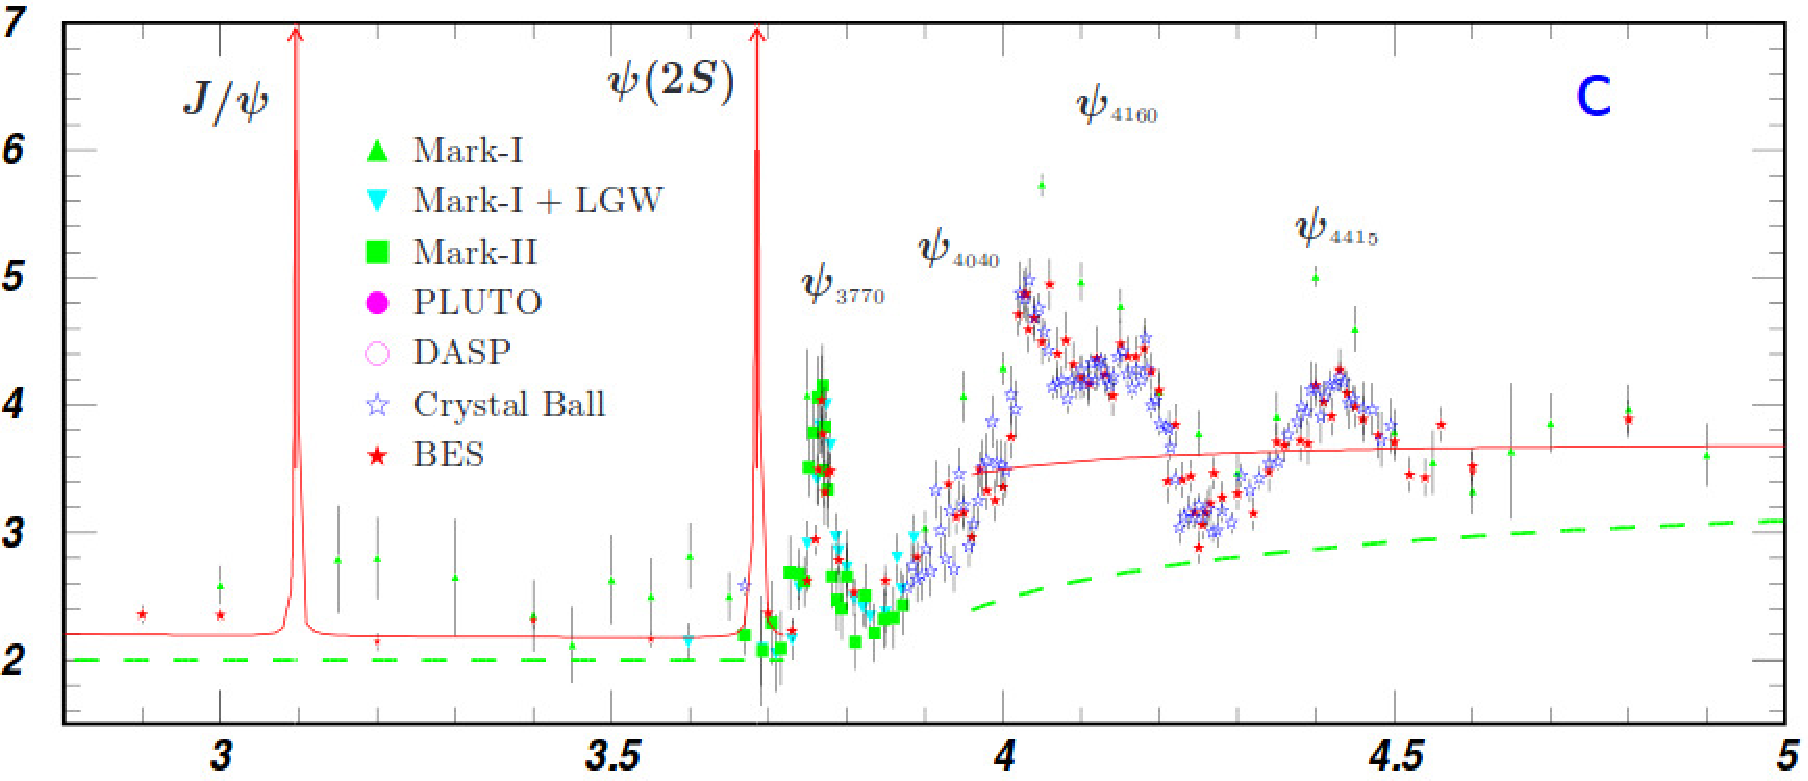
\includegraphics[scale=0.50]{figures/images/R_scan.pdf}
\caption{Measurements of $R = \sigma(\ee \rightarrow \text{hadrons}) / \sigma(\ee \rightarrow \mumu)$.}
\label{fig:R_scan}
\end{figure}

Many of the lower mass resonances are predictable within the context of the quark model.
However, there are a number of states which have been predicted, but not yet discovered.
There are also states which were discovered experimentally without any corresponding predictions.
A variety of these particles are shown in \Cref{fig:charmonia}.

\begin{figure}[H]
\centering
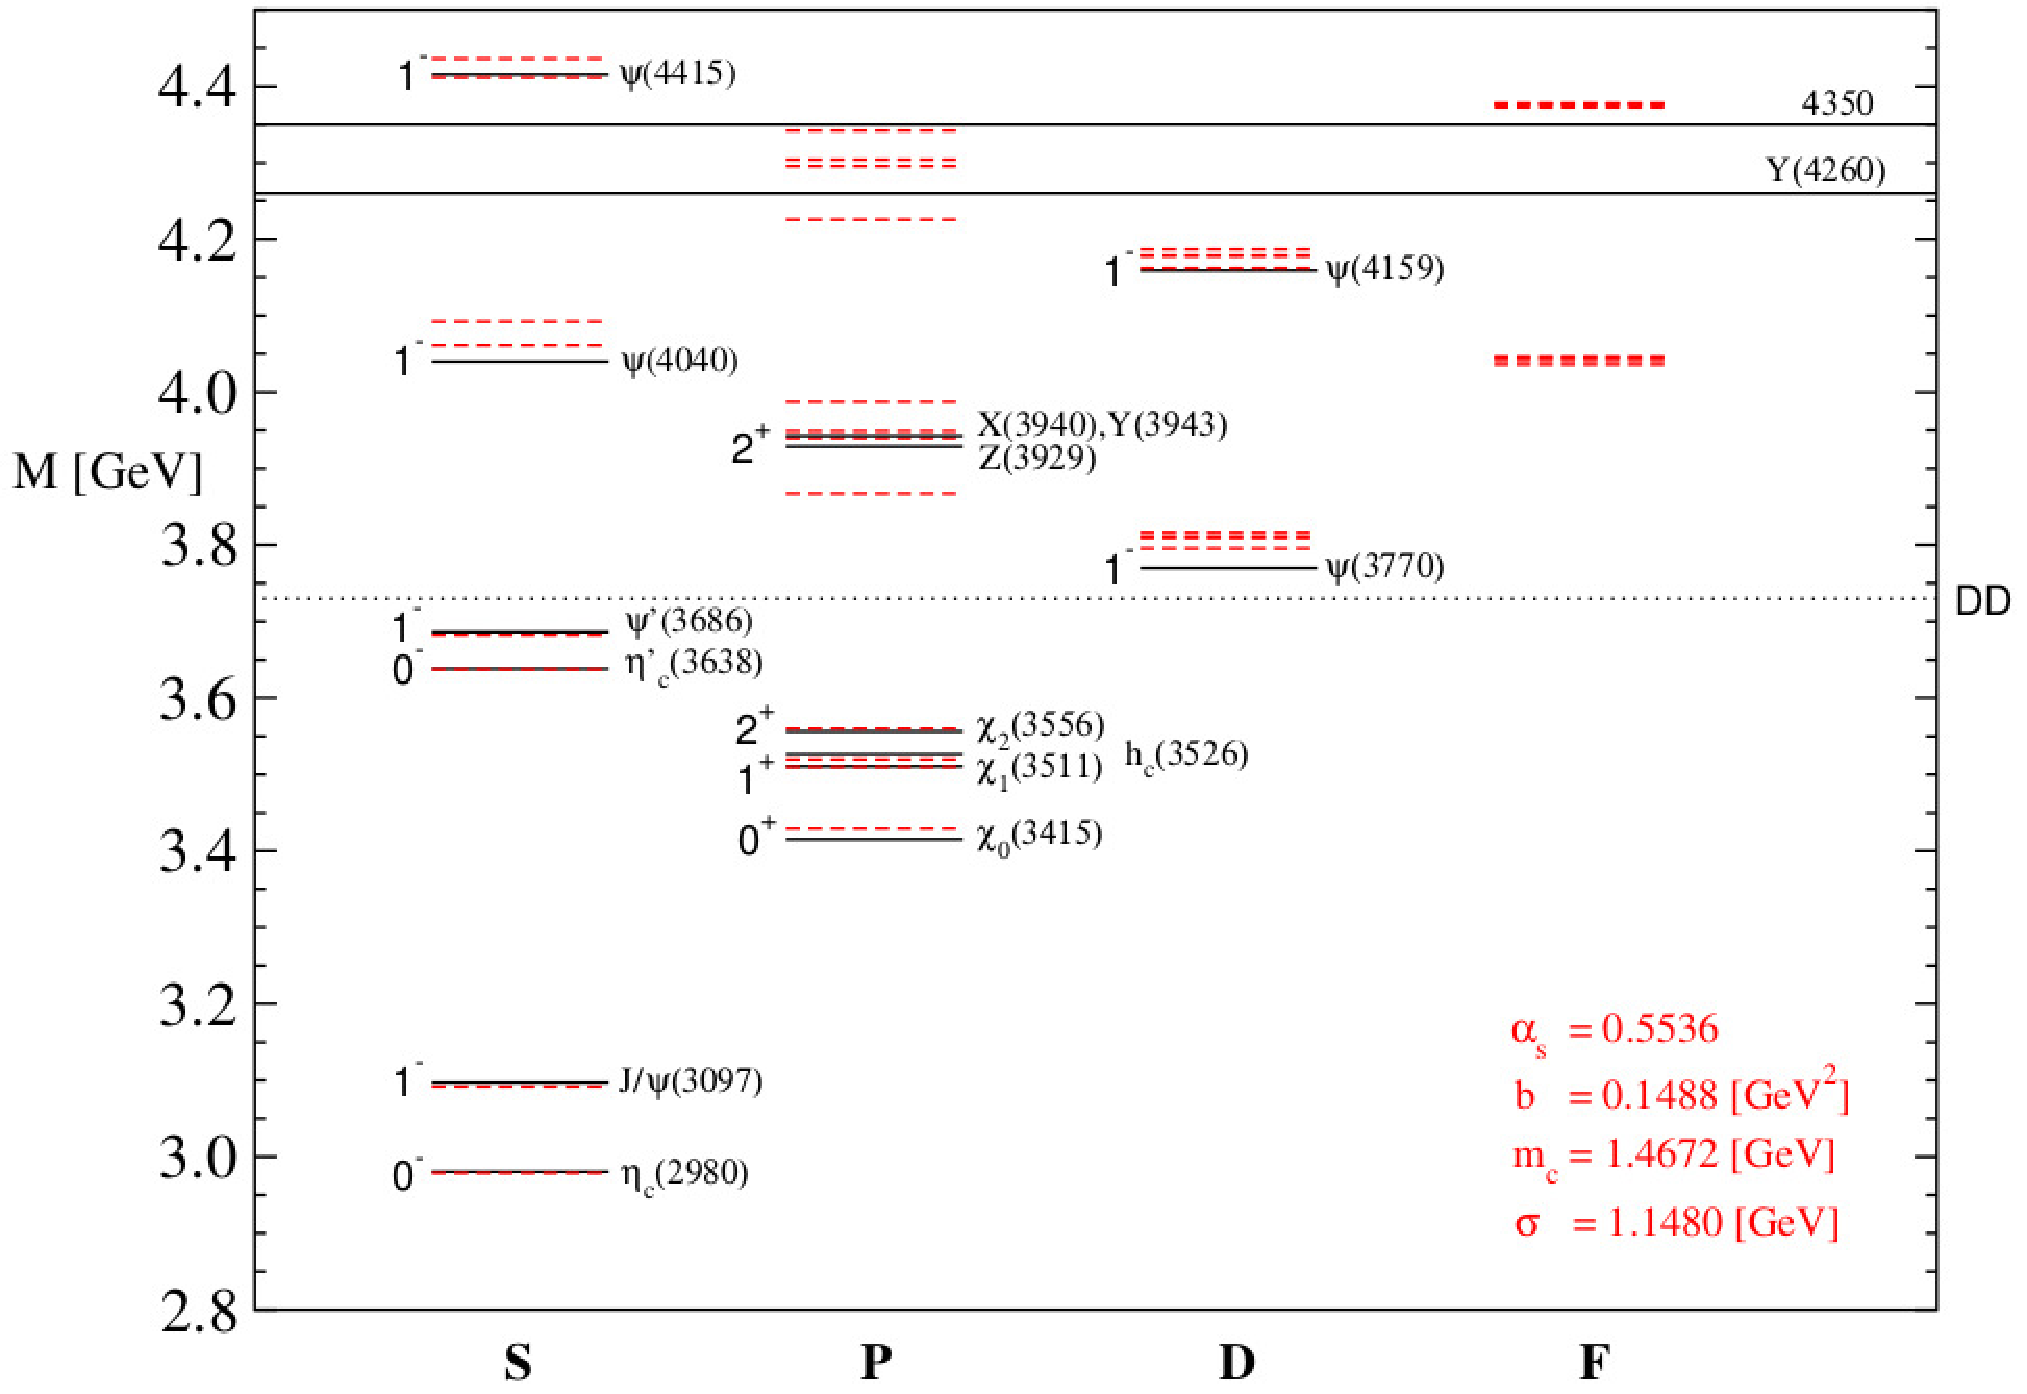
\includegraphics[scale=0.40]{figures/images/charmonia.pdf}
\caption{Measured and predicted charmonium resonances.}
{Solid black lines represent measurements while the dashed red lines are predictions.}
\label{fig:charmonia}
\end{figure}

The resonances below the $\DDbar$ threshold, like the $\jpsi$ and the $\psip$, show solid agreement with their theoretical predictions.
However, many of the ones above, such as the $\psipp$, still show some disagreement.
This is likely due to the more complicated interactions introduced from $\DDbar$ decays.
Several experiments have attempted to measure the shape of the $\psipp$ based on different assumptions.
The most prominent of these is the assumption of interference.
This can have notable effects on the resultant parameters of the $\psipp$, such as the mass, shown in \Cref{tab:previous_results}.

\begin{table}[H]
\centering
\begin{tabular}{c l|c l}
\hline
\multicolumn{2}{c|}{$\Mpsipp$ [\si{\MeV}] (No Interference)} & \multicolumn{2}{c}{$\Mpsipp$ [\si{\MeV}] (With Interference)} \\ [1pt] 
\hline
BES-II \cite{ref:Ablikim:2007}   & 3772.0 $\pm$ 1.9           & BaBar \cite{ref:Aubert:2008b} & 3778.8 $\pm$ 1.9 $\pm$ 0.9 \\
Belle  \cite{ref:Brodzicka:2008} & 3776.0 $\pm$ 5.0 $\pm$ 4.0 & KEDR  \cite{ref:Anashin:2012} & $3779.2^{+1.8 \, +0.5 \, +0.3}_{-1.7 \, -0.7 \, -0.3}$ \\ 
BaBar  \cite{ref:Aubert:2008a}   & 3775.5 $\pm$ 2.4 $\pm$ 0.5 & & \\
\hline
\end{tabular}
\caption{Previous experimental results for the mass of the $\psipp$.}
{Where applicable, the first errors are statistical, the second are systematic, and the third are model-dependent.}
\label{tab:previous_results}
\end{table}

Both BaBar \cite{ref:Aubert:2008b} and KEDR \cite{ref:Anashin:2012} found it necessary to include interference effects for fitting the $\DDbar$ spectrum.
However, the statistics of the KEDR sample were insufficient to fully resolve the discrepancies seen with other experiments that ignored interference.
{\bf Using the larger data sample available at BESIII, we have precisely measured and analyzed the shape of the $\DDbar$ spectrum around the $\psipp$ resonance.}
We have also used this measurement to probe the branching fraction of $\nonDDbar$ decays in this region.


To begin this analysis, we provide background on relevant theoretical concepts and derivations.
Next, we detail specifications for the collider and detector which collected the data used for these measurements along with their related analysis software and reconstruction methods. 
From here, we describe the procedure for determining the $\psipptoDD$ cross section and show the results with systematic uncertainties.
Finally, we examine the current progress of measuring the $\nonDDbar$ branching fraction.

